\documentclass[notoc,justified]{tufte-book}    % `notoc` suppresses TL custom TOC, reverts to standard LaTeX
\usepackage{graphicx}
\hyphenation{HMMER}

\title{User's Guide for the HMMER Daemon}

\subtitle{High-performance biological sequence analysis using profile hidden Markov models}

\author{Sean R. Eddy, Nicholas P. Carter}
\subauthor{and the HMMER development team}

\pkgurl{http://hmmer.org}
\pkgversion{3.3.2}   % ./configure replaces HMMER_VERSION
\pkgdate{Nov 2020}         %    ... and HMMER_DATE

                    % definitions for \maketitle 
\bibliographystyle{unsrtnat-brief}   % customized natbib unsrtnat. Abbrev 3+ authors to ``et al.'' 

\begin{document}
\setcounter{tocdepth}{2}             % 0=chapters 1=sections 2=subsections 3=subsubsections? 4=paragraphs
\newcommand{\UNIrelease}{2020\_05}
\newcommand{\UNInseq}{563,552}

\newcommand{\HMMERversion}{3.3.2}
\newcommand{\HMMERdate}{Nov 2020}

\newcommand{\BGLnseq}{4}
\newcommand{\BGLalen}{171}
\newcommand{\BGLmlen}{149}
\newcommand{\BGLgaps}{22}
\newcommand{\BGLeffn}{0.96}
\newcommand{\BGLre}{0.589}

\newcommand{\HMMERfmtversion}{f}
\newcommand{\HMMERsavestamp}{[3.3.2 | Nov 2020]}

\newcommand{\SGUevalue}{4.9e-65}
\newcommand{\SGUbitscore}{223.2}
\newcommand{\SGUbias}{0.1}
\newcommand{\SGUorigscore}{223.3}
\newcommand{\SGUdombitscore}{223.0}
\newcommand{\SGUseqname}{HBB\_GORGO}
\newcommand{\SGUmsvpass}{3.7}
\newcommand{\SGUbiaspass}{17002}
\newcommand{\SGUvitpass}{2323}
\newcommand{\SGUfwdpass}{1129}
\newcommand{\SGUelapsed}{0.9}

\newcommand{\SFSevalue}{5.6e-57}
\newcommand{\SFSbitscore}{176.4}
\newcommand{\SFSdomevalue}{2.3e-16}
\newcommand{\SFSdombitscore}{46.2}
\newcommand{\SFSexpdom}{9.8}
\newcommand{\SFSndom}{9}

\newcommand{\SFSmaxdom}{7}
\newcommand{\SFSmaxdomu}{5}
\newcommand{\SFSmaxsc}{46.2}
\newcommand{\SFSievalue}{2.3e-16}
\newcommand{\SFSuievalue}{1.3e-10}
\newcommand{\SFSdomZ}{794}
\newcommand{\SFSucevalue}{1.9e-13}
\newcommand{\SFSaidx}{1}
\newcommand{\SFSascore}{-1.9}
\newcommand{\SFSaevalue}{0.24}
\newcommand{\SFSauevalue}{191}
\newcommand{\SFSacoords}{395-410}
\newcommand{\SFSbidx}{6}
\newcommand{\SFSbscore}{0.4}
\newcommand{\SFSbevalue}{0.045}
\newcommand{\SFSbuevalue}{35.7}
\newcommand{\SFSbcoords}{1742-1769}
\newcommand{\SFSainsig}{4.6}
\newcommand{\SFSbinsig}{8.9}

\newcommand{\JHUninc}{955}
\newcommand{\JHUnsig}{955}

\newcommand{\NMHafrom}{302390}
\newcommand{\NMHato}{302466}
\newcommand{\NMHbfrom}{302466}
\newcommand{\NMHbto}{302389}
\newcommand{\NMHnres}{660000}
\newcommand{\NMHntop}{330000}
\newcommand{\NMHnssv}{73493}
\newcommand{\NMHfracssv}{11.1}
\newcommand{\NMHnbias}{49311}
\newcommand{\NMHfracbias}{7.5}
\newcommand{\NMHnvit}{4022}
\newcommand{\NMHfracvit}{0.6}
\newcommand{\NMHnfwd}{1562}
    % snippets captured from output, by gen-inclusions.py 

\maketitle

\newpage
\vspace*{\fill}
\begin{flushleft}

\vspace{2em}
Copyright (C) 2020 Howard Hughes Medical Institute.

\vspace{2em}
Infernal and its documentation are freely distributed under the 
3-Clause BSD open source license. For a copy of the license, see
\url{http://opensource.org/licenses/BSD-3-Clause}.

\vspace{2em}
Infernal development is supported by the Intramural Research Program
of the National Library of Medicine at the US National Institutes of
Health, and also by the National Human Genome Research Institute of
the US National Institutes of Health under grant number
R01HG009116. The content is solely the responsibility of the authors
and does not necessarily represent the official views of the National
Institutes of Health.

\end{flushleft}






\begin{adjustwidth}{}{-1in}          % TL \textwidth is quite narrow. Expand it manually for TOC and man pages.
\tableofcontents                     
\end{adjustwidth}


\chapter{Introduction}

The performance of HMMER's command-line tools is limited by two factors: the number of cores that are available to work on each search, and the amount of time required to read sequence or HMM databases from disk in order to search them.  When HMMER is run on small (2- or 4-core) desktop or laptop CPUs, CPU performance tends to be the limiting factor on search time (although this depends on the speed of the system's hard disk).  However, on systems with more cores, such as most servers, the time required to read databases from disk becomes a bottleneck that prevents performance from improving as processor performance increases.

To address this, HMMER provides a  daemon\sidenote{The term "daemon" here is taken from the UNIX term for an application or service that runs without being connected to a user login, which is derived from a Greek term that means roughly "spirit" or "supernatural being".}, known as \mono{hmmpgmd}  that runs as a persistent service across multiple computers.  As shown in Figure \ref{fig:daemon}, one machine running the daemon is designated the master node, while the others become worker nodes.  Client systems send search requests to the master node via internet sockets.  When the master node receives a search, it distributes the work of the search across the worker nodes, merges the partial results from each worker node, and returns the search results to the client\sidenote{In the European Bioinformatics Institute's (EBI) instantiation of the daemon, the client machines shown in the figure are EBI's web servers.  End users interact with the web servers, which provide a human-friendly interface for submitting searches and inspecting results.}.

\begin{figure*}
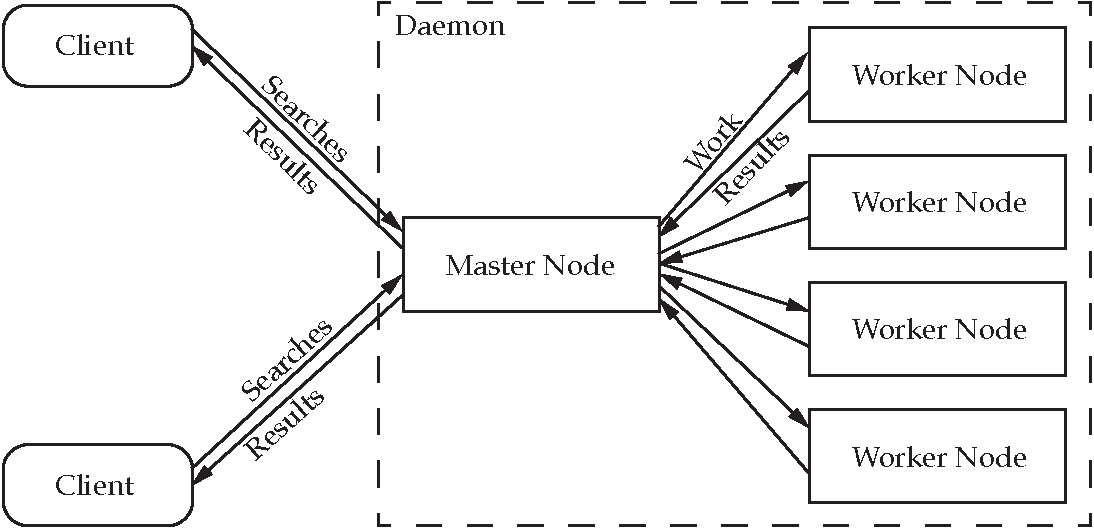
\includegraphics[width=\textwidth]{inclusions/daemon.pdf}
\caption{The HMMER Daemon}
\label{fig:daemon}
\end{figure*}

The daemon improves search performance over HMMER's command-line tools in two ways.  First, when the daemon starts up, it reads its input databases from disk once and caches them in RAM, eliminating the file read bottleneck on performance.  Second, it distributes the work of each search over many machines, each of which may contain tens of cores, significantly reducing the amount of work each core must perform to complete the search.  In combination, these techniques can reduce database search times to only a few seconds when the daemon is run on a large-enough set of computers.  

\mono{Hmmpgmd} caches all of its database(s) in RAM on each of its worker nodes, in spite of the fact that each worker node only accesses part of a database on each search.  This allows \mono{hmmpgmd} to tolerate worker node failures by simply changing how work is assigned to the worker nodes as the number of worker nodes changes, but causes \mono{hmmpgmd} to use significantly more memory than would be strictly necessary, particularly when the daemon has many worker nodes.  To address this, HMMER now provides a "sharded" version of \mono{hmmpgmd}, \mono{hmmpgmd\_shard}, which distributes the sequences in a sequence database\sidenote{We do not support sharding of HMM databases because current HMM databases are so much smaller than current sequence databases that the amount of RAM they occupy has not been an issue.} round-robin across the worker nodes so that each worker node only caches $\frac{1}{Nth}$ of each sequence database.  This allows systems with limited RAM to support larger sequence databases, at the cost of making the daemon unable to execute searches unless all of its worker nodes are available.

\mono{Hmmpgmd} was designed to be integrated with the European Bioinformatics Institute's computing and database infrastructure.  To reduce RAM and bandwidth usage, sequence names, accession information, and descriptions are not included in \mono{hmmpgmd's} databases and are not cached in RAM.  Instead, each sequence or HMM is assigned an ID number based on its position in the database file, and \mono{hmmpgmd} reports that ID number when a hit occurs.  EBI's web servers then look that ID number up in their own databases to retrieve the sequence/HMM's name, description, etc., and combine that with the alignment information the daemon returns when displaying search results to users.

This manual outlines \mono{hmmpgmd}'s usage and interface to client applications, and assumes that the reader is familiar with the concepts covered in the main \underline{HMMER User's Guide}.  It is intended for individuals who are interested in either running an \mono{hmmpgmd} server of their own or in writing clients that communicate with an existing \mono{hmmpgmd} server.   Biologists who wish to use an \mono{hmmpgmd} server in their research without the complexity of configuring one themselves should consider using the European Bioinformatics Institute's HMMER server\sidenote{www.ebi.ac.uk/Tools/hmmer/}, which provides a web interface to \mono{hmmpgmd} servers that load a number of common genetic databases.
 

\chapter{Usage}
To perform searches using \mono{hmmpgmd}, a user must first start a daemon on one or more machines.  At least two \mono{hmmpgmd} processes, one master and one worker, must be started, although these processes may be run on the same computer if only one machine is available\sidenote{When running \mono{hmmpgmd} on a single machine, be aware that the master and worker processes will load the database(s) into RAM independently, so the memory required will be approximately double what is required when running the worker and master processes on separate machines.  \mono{Hmmpgmd\_shard} greatly reduces the amount of memory used by the master node, so using it with only one shard may be a better choice for searching sequence databases on a single machine.}.  Once the daemon is running, users can submit searches via a client program such as the \mono{hmc2} example client HMMER provides.

\section{Running Hmmpgmd}
To start a daemon process, execute the "\mono{hmmpgmd}" command.  \mono{Hmmpgmd} requires that the user provide either the \mono{-{}-master} flag, which indicates that the process should run as the master node of a daemon, or the \mono{-{}-worker <IP of master node>}, which indicates that \mono{hmmpgmd} should run as a worker node with its master node at the specified IP address\sidenote{If the master node's IP is omitted, \mono{hmmpgmd} defaults to connecting to a master process on the same node it is running on.}.  Note that this IP address must be provided as a numeric value, for example "127.0.0.1", and not as a text machine name, as \mono{hmmpgmd} does not perform domain name service lookup on the provided IP address.  

When run as a master node, \mono{hmmpgmd} requires that the user provide at least one of the \mono{-{}-seqdb <filename>}, or \mono{-{}-hmmdb <filename>} options to specify a sequence and/or HMM database for the daemon to cache in RAM.  The user may specify both a sequence and an HMM database file that the daemon should cache.  The master node reads the database(s) itself and also sends the specified filename(s) to each of the worker nodes so that they can cache their own copies of the database(s).  Thus, the database file(s) must be available on all of the nodes in the daemon and the filename(s) provided must be valid paths to the database file(s) on all of the nodes, either because \mono{hmmpgmd} is invoked from the same directory on every node or because the filename(s) are specified as full paths from the root node of the filesystem.

When run as a master node, \mono{hmmpgmd} first reads its input databases and then listens for socket connections from worker nodes.  When a worker node connects to the master, the master outputs  "Handling worker <IP address (socket number)"" to its display or logfile.  After the worker has read its databases and is ready to handle work, the master outputs "Pending worker <IP address> (socket number)".  The master can begin accepting search requests from clients as soon as one worker node has reached the pending state, and will distribute each search across all of the worker nodes that are pending when the search begins.


\subsection{Running \mono{hmmpgmd\_shard}}
Starting a sharded daemon using the \mono{hmmpgmd\_shard} program follows the same procedure as starting an undsharded daemon, with two exceptions.  First, when run on the master node \mono{hmmpgmd\_shard} takes a mandatory \mono{--num\_shards <n>} argument, which specifies the number of shards that the sequence database file should be broken into.  This must be equal to the number of worker nodes that will connect to the master.  Second, because each worker node only contains a portion of its sequence database(s), \mono{hmmpgmd\_shard} can only process search requests when the number of worker nodes connected to it is equal to the number of shards.  Attempting to run searches before that many worker nodes have connected will return an error.  Attempting to connect more worker nodes than the specified number of shards causes the daemon to exit.

Note that \mono{hmmpgmd\_shard} only shards sequence databases.  HMM databases are not sharded, due to their small size, so there is no reason to use \mono{hmmpgmd\_shard} on HMM databases. 


\section{Sending Searches to a Daemon}
The HMMER package includes {\em hmmc2}, an example client that can communicate with an \mono{hmmpgmd} or \mono{hmmpgmd\_shard} daemon.  Hmmc2 accepts four command-line arguments\sidenote{Hmmc2's code breaks Easel conventions by manually parsing its command-line arguments instead of using Easel's \mono{getopts} functions.  It also defines a separate Easel \mono{getopts} structure, \mono{{searchOpts}}, which it uses to parse search requests, which can easily be mistaken for a definition of \mono{hmmc2's} command-line options.}:

\begin{sreitems}{\monob{header}}
  \item[\monob{-i <IP address>}] specifies the IP address of the daemon to connect to.  Defaults to 127.0.0.1 if not provided.
  \item[\monob{-p <port>}] specifies the port number that the daemon is listening to for client connections.  Defaults to 51371 (the \mono{hmmpgmd} default) if not provided.
  \item[\monob{-S}] print the scores of any hits found by searches
  \item[\monob{-A}] print the alignments of any hits found by searches.  The data printed when this option is provided is a superset of the data printed when "-S" is provided, so the "-S" option is redundant if -A is provided.
\end{sreitems}

Once it starts up, \mono{hmmc2} enters an interactive loop by printing the prompt "Enter next sequence:".  Any text the user enters between that prompt and the end-of-command string "{\tt //}" is interpreted as a command and sent to the daemon.  

\subsection{Usage Example}
After starting \mono{hmmc2} with the command

\vspace{1ex}
\user{hmmc2 -i <IP of daemon's master node>}
\vspace{1ex}

it will print the prompt

 \vspace{-1ex}
  \xsreoutput{inclusions/hmmc2.out}
 \vspace{-1ex}

To run a simple search, enter the text

\vspace{1ex}
\user{@-{}-seqdb 1} \\
\user{>sp|Q6GZW9|length\_10} \\
\user{YLGPWVQAEY} \\
\user{//}
\vspace{1ex}

The text {\small\bfseries\texttt @-{}-seqdb 1} on the first line instructs the daemon to perform a search against sequence database 1. The next two lines ({\small\bfseries\texttt >sp|Q6GZW9|length\_10} and {\small\bfseries\texttt YLGPWVQAEY}) are the FASTA-format specification of a (short) amino acid sequence that the daemon will translate into an HMM and search against the database.  Finally, the 
{\small\bfseries\texttt //} by itself on the third line ends the command.  

Once it sees the end-of-command sequence, \mono{hmmc2} will send the command to the server, which will perform the search and generate output similar to

\vspace{-1ex}
  \xsreoutput{inclusions/hmmc2_2.out}
 \vspace{-1ex}

 although the exact output generated will vary depending on the database that the daemon has cached.  This output is a simple summary that shows the number of comparisons performed by the daemon, the number of hits found, and the time it took to perform the search.  If the \mono{-S} or \mono{-A} options had been used when starting \mono{hmmc2}, substantially more information about the hits found by the server would have been displayed.

 The next chapter provides significantly more detail about the format of the commands the daemon accepts and of the output it sends back to the client.

\chapter{Daemon-Client Interface}
Client machines use internet sockets to send commands to and receive results from a daemon's master node.  When a client opens a connection to the master node's client communication port (port 51371 by default), the master node forks a thread to manage the connection with the client.  This thread configures a socket to communicate with the client and then repeatedly calls the \mono{clientside\_loop}\sidenote{This function name is a bit of a misnomer, in that it does not contain a loop.  Instead, it is repeatedly called from within an outer loop.} function, which monitors the socket for commands from the client, until either the client detaches from the port or the daemon shuts down.  This approach allows multiple clients to connect to a daemon simultaneously without interfering with each other, although requests from one client may impact the amount of time it takes for the daemon to respond to requests from other clients.


\section{Daemon Command Format}
Daemon commands are variable-length sequences of ASCII text.  The first line of a command must contain the command itself and any options or parameters.  For search commands, this is followed by one or more lines that contain the sequence or HMM to be searched.  All commands end with a line that contains only two forward slashes ("{\tt //}").  When a command arrives from a client, the daemon reads bytes from the appropriate socket into a buffer until it sees the end-of-command sequence, growing the buffer as necessary\sidenote{This is a security vulnerability that should be addressed in HMMER4, as it allows an adversarial or erroneous client to consume arbitrary amounts of RAM, potentially exceeding the capacity of the master node.}, and then parses the contents of the buffer in order to execute the command.   

The daemon supports three commands:

\begin{sreitems}{\monob{header}}
  \item[\monob{@-{}-hmmdb <database \#>}]  Initiates a search of a protein sequence against the HMM database cached by the daemon.  The protein sequence to be searched must be provided on the lines following the \mono{@-{}-hmmdb} command.  Note that the user is required to provide a database number argument to \mono{@-{}-hmmdb}, but \mono{hmmpgmd} can only load one HMM database at a time and ignores the value provided.  This is a known idiosyncrasy that has been left unchanged to avoid breaking EBI's tools and web interface code.
  \item[\monob{@-{}-seqdb <database \#> [-{}-seqdb\_ranges <rangelist>]}] Initiates a search of a protein sequence or HMM against the specified protein sequence database\sidenote{Note that there is an inconsistency in how databases are numbered in search commands as compared to how they are numbered in the database file itself.  The database file uses 0-indexed numbering, (databases are numbered from 0 to N-1), while the search commands use 1-indexed numbering (databases are numbered from 1 to N)}.  The daemon determines whether a sequence or HMM has been submitted by examining the contents of the lines that follow the command, and, if a sequence has been submitted, converts it to an HMM before performing the search.

  If the \mono{-{}-seqdb\_ranges} option is not provided, the entire target database is searched\sidenote{Currently, there is no way to search only a portion of an HMM database.  This is probably because existing HMM databases are small enough that the time to search them is rarely an issue.}. If the \mono{-{}-seqdb\_ranges} option is provided, it must be followed by a range list describing the set of sequences to be searched.  Each range in the range list should be formatted in the form "start..end", where "start" and "end" are the sequence IDs of the start and end of the range, and ranges in the list should be separated by commas. One note here is that the sequences in a sequence file are indexed as a single contiguous list, even if the file contains multiple databases, and each database can contain an arbitrary subset of the sequences in the file.  Thus, the sequence IDs specified in a range list refer to positions within the database file, and a range list search searches the sequences in the specified database whose IDs fall into the specified range(s), not the specified positions in the set of sequences contained in the database. For example: the command {\small\bfseries\texttt @-{}-seqdb 2 -{}-seqdb\_ranges 1..100, 201..300} searches the sequences in database 2 whose sequence ID's range from 1 to 100 or 201 to 300, not sequences 1-100 and 201-300 of the database.
  \item[\monob{!shutdown}] Shuts the daemon down in an orderly fashion by first sending shutdown messages to all of its worker nodes and then exiting the master node's processes\sidenote{There's another security vulnerability here, in that any machine that can connect to the master node can shut it down.  This needs to be addressed in H4, as we intend to allow arbitrary clients to send searches to a server}.
\end{sreitems}

When the daemon receives a search command, any text on the command line after the \mono{@-{}-seqdb <database \#>} or \mono{@-{}-hmmdb <database \#>} specifies options to the search, using the same format as the \mono{hmmsearch} or \mono{hmmscan} commands.  Thus sending the command \user{@-{}-seqdb 1 -E 20} to the daemon instructs it to perform a search of sequence database 1, reporting all results with an e-value of less than 20 instead of the default 10.


\section{Search Results Format}
The results from each search are split across two sockets messages, as shown in Figure \ref{fig:search-results}.  The first is a fixed-length \mono{HMMD\_SEARCH\_STATUS} structure that contains two fields: a \mono{status} field that contains an Easel status code that tells the client whether the search completed successfully or not, and a \mono{msg\_size} field, which tells the client how large (in bytes) the second message will be.  The format of the second message depends on whether any errors were encountered during the search.  If an error occurred, the second message is simply a text string containing a description of the error.  


\begin{figure*}
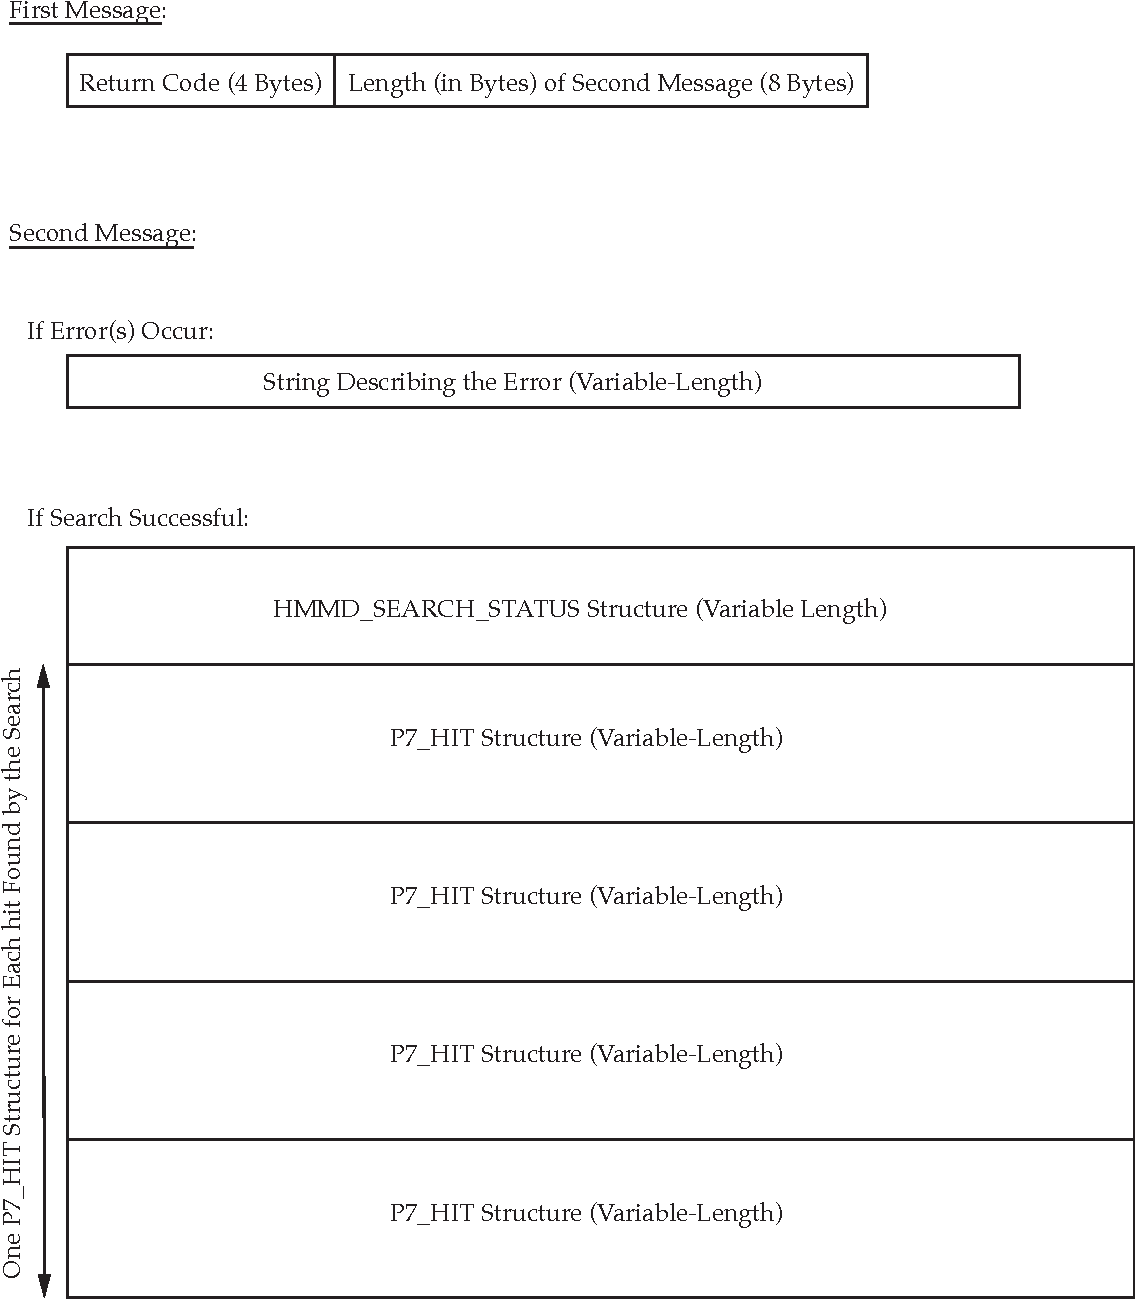
\includegraphics[width=\textwidth]{inclusions/daemon-results.pdf}
\caption{Format of the Messages the Daemon Sends to a Client When a Search Completes}
\label{fig:search-results}
\end{figure*}

If the search succeeded, the \mono{status} field of the first message is set to \mono{eslOK} and the second message contains the results of the search.  This message begins with a \mono{HMMD\_SEARCH\_STATS} structure that contains information about the search, including the time the search took and the number of hits found.  This is then followed by a \mono{P7\_HIT} structure for each hit the search found, which describes the hit.

\section{Serialization}
Data structures and multi-byte values must be {\em serialized} before they can be sent over sockets.  There are two aspects to serializing the types of data structures the daemon uses.  Structures that contain pointers must be {\em flattened} by copying the data that their pointers point to into the block of data that will be sent over the socket, and multi-byte values must be converted to "network order," which is defined as big-endian, to prevent problems if the sending and receiving machines have different endiannesses.  To serialize floating-point numbers, we assume that all computers use IEEE 754 representations and just convert the bytes that represent the floating-point number to and from network byte order.  This is faster than the alternative approach of representing the floating-point number as an ASCII string and parsing it on the receiving side, and avoids any loss of precision, but will fail if the machines trying to communicate via sockets use different floating-point formats.  

Figures \ref{fig:search-stats-serialize}--\ref{fig:alidisplay-serialize} show how the data structures used in sending search results back to clients are serialized.  The text streams the client uses to send commands to the daemon do not require serialization, as text streams do not contain pointers and are sequences of byte-wide characters that are not affected by endianness.    

\begin{figure*}
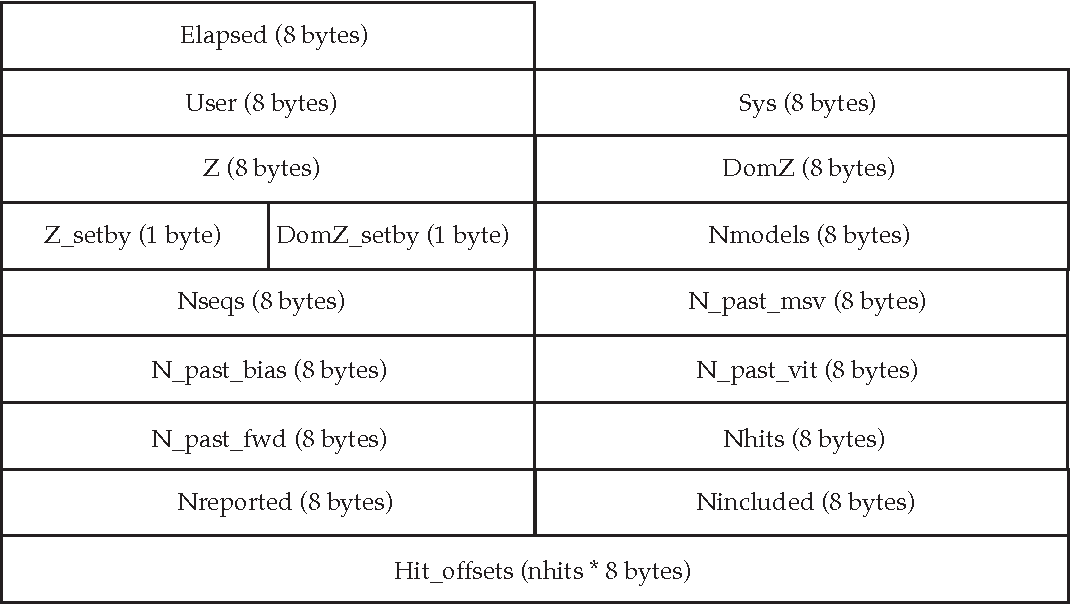
\includegraphics[width=\textwidth]{inclusions/hmmpgmd-search-stats-serialize.pdf}
\caption{Serialized {HMMD\_SEARCH\_STATS} Structure}
\label{fig:search-stats-serialize}
\end{figure*} 

\begin{figure*}
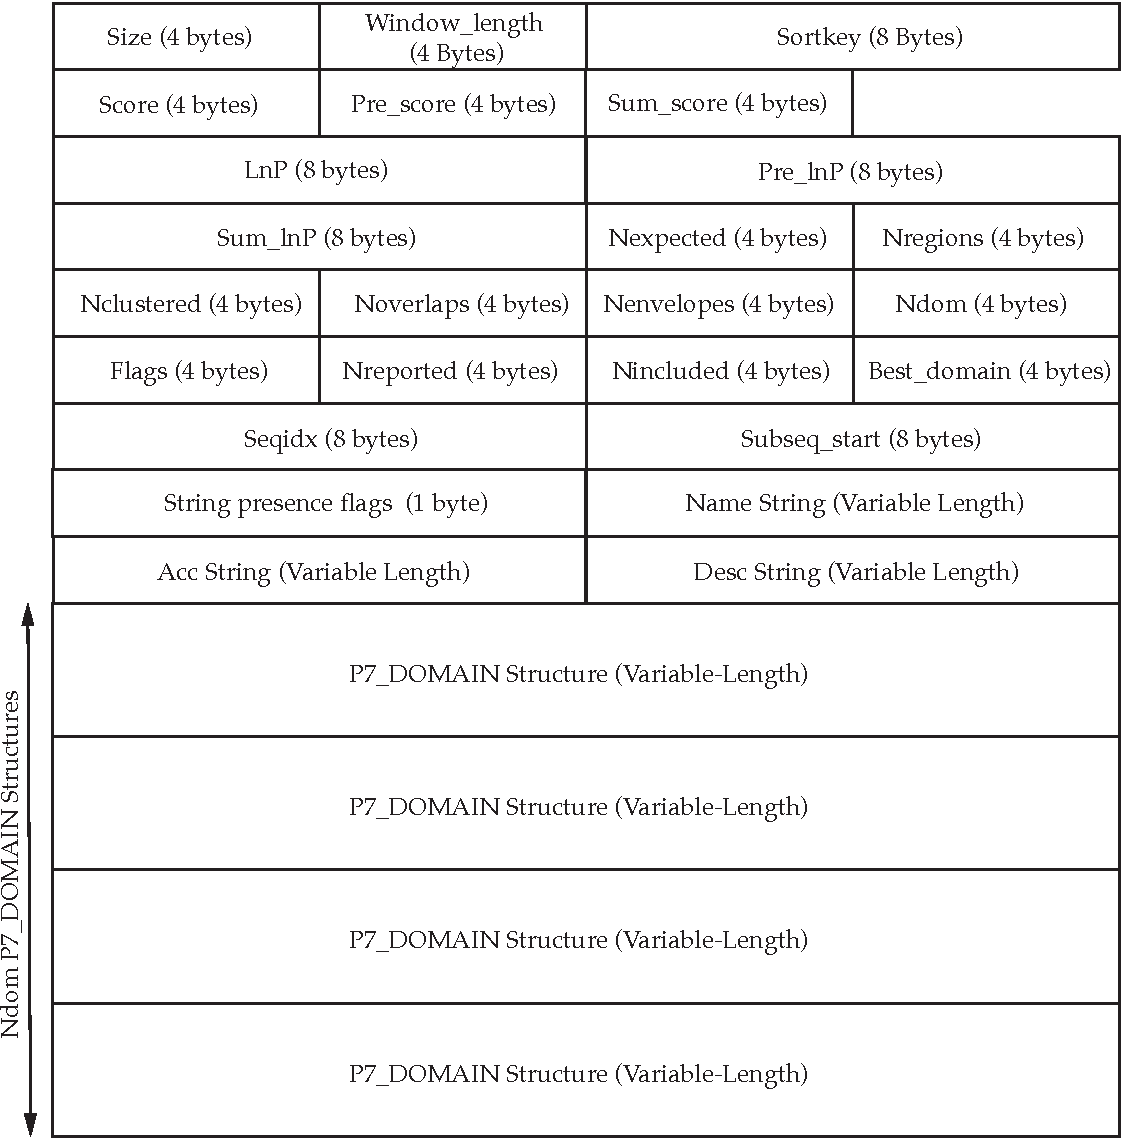
\includegraphics[width=\textwidth]{inclusions/hit-serialize.pdf}
\caption{Serialized {P7\_HIT} Structures}
\label{fig:hit-serialize}
\end{figure*}
\begin{figure*}
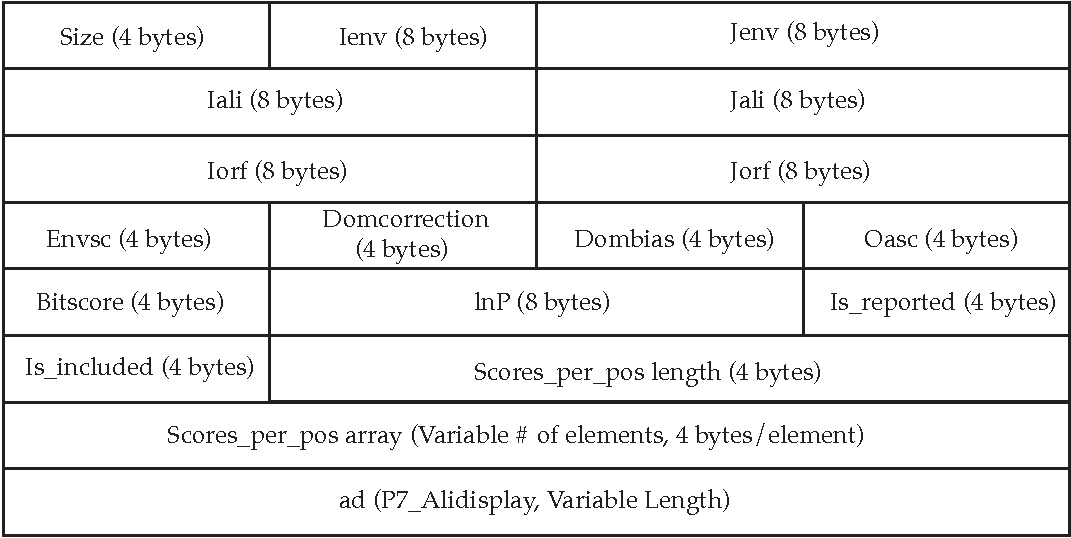
\includegraphics[width=\textwidth]{inclusions/domain-serialize.pdf}
\caption{Serialized {P7\_DOMAIN} Structure}
\label{fig:domain-serialize}
\end{figure*}
\begin{figure*}
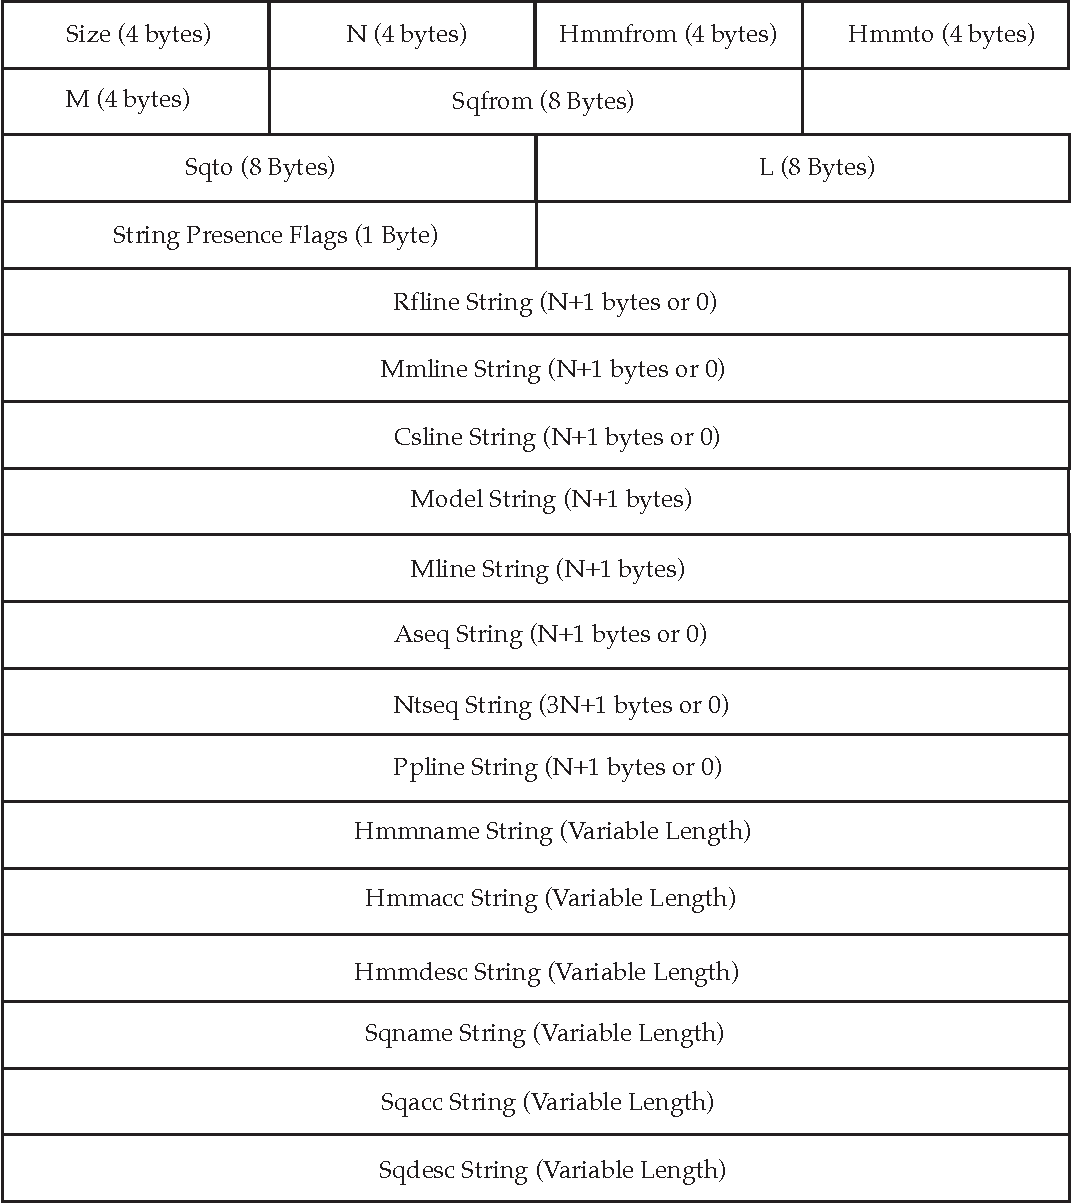
\includegraphics[width=\textwidth]{inclusions/alidisplay-serialize.pdf}
\caption{Serialized {P7\_ALIDISPLAY} Structure}
\label{fig:alidisplay-serialize}
\end{figure*}

All of the data structures that hmmpgmd serializes contain variable-length fields, and many of them contain optional fields that may or may not be present in a given object.  We handle optional fields by adding a byte of presence bit flags, one flag per optional field, to the serialized versions of data structures that contain optional fields.  If the flag bit corresponding to a field is set, then that field is present in the data structure. Otherwise it is not present.  None of the data structures hmmpgmd serializes have more than eight optional fields, so only one byte of presence flags/structure is required.

Most of the variable-length fields in our data structures are strings, which we represent as standard C-terminated strings.  Routines such as \mono{strcpy} are used to copy these strings into and out of the serialized data structures, making it unnecessary to encode the strings' length in the serialized data structure.  Some non-string fields, such as the \mono{hit\_offsets} field in the {\mono{HMMD\_SEARCH\_STATS}} structure, have lengths that are determined by the value of some other field in the data structure, so it is not necessary to explicitly encode their lengths in the serialized data structures. One field, the \mono{scores\_per\_pos} array in the {\mono{P7\_DOMAIN}} structure, has a length that cannot be determined from the other data in the data structure, so we add an explicit field to the serialized data structure to encode its length.

Because it is sometimes necessary to manipulate serialized data without deserializing the full set of results, we include two mechanisms to help locate sub-fields of the daemon's results.  The {\mono{HMMD\_SEARCH\_STATS}} structure contains a \mono{hit\_offsets} array that contains the offsets from the start of the block of serialized hits to the beginning of each serialized hit.  Also, all of our serialized data structures except {\mono{HMMD\_SEARCH\_STATS}} begin with a \mono{size} field that contains the length of the base (i.e., without any included sub-structures) serialized data structure in bytes.  For example, the \mono{size} field of a {\mono{P7\_HIT}} structure will contain the length of the serialized {\mono{P7\_HIT}} structure not including the lengths of the {\mono{P7\_DOMAIN}} structures that the {\mono{P7\_HIT}} structure contains.  These features allow software to quickly locate a specific {\mono{P7\_HIT}} structure within the array of results after decoding the {\mono{HMMD\_SEARCH\_STATS}} structure, and then to skip through the {\mono{P7\_HIT}} structure as necessary to locate its sub-fields.

Functions to serialize and deserialize each of the daemon's data structures are provided in the .c files that contain the structure's routines.     

\chapter{Database File Formats}
The formats \mono{hmmpgmd} uses for HMM and sequence databases are derived from the formats used elsewhere in HMMER, with modifications to support integration with EBI's infrastructure and reduce the size of sequence databases.

\section{HMM Database File Format}
\mono{hmmpgmd} uses the HMMER 3 profile HMM file format as described in the \underline{HMMER User's Guide} for its HMM databases, with the requirement that the HMM file must have been processed by \mono{hmmpress} before it can be loaded into \mono{hmmpgmd}.  When an HMM database is cached in RAM, it is represented as a simple array of \mono{P7\_OPROFILE} objects, although each HMM's name is replaced with its ID number (position in the database file).  Each HMM file can only contain a single HMM database, and \mono{hmmpgmd} does not support caching of multiple HMM databases simultaneously.

\section{Sequence Database File Format}
The \mono{hmmpgmd} format that \mono{hmmpgmd} uses for sequence database files is a variant of the FASTA format in which sequence names are replaced with numeric IDs, sequence descriptions and accession information are removed, and new sequence descriptions are added that enable efficient caching of multiple databases simultaneously and assist EBI's web servers.  
A FASTA file can be converted into a single-database \mono{hmmpgmd} sequence file using the \mono{esl-reformat} command.  For example, 

\user{esl-reformat --id\_map mydb.hmmpgmd.map hmmpgmd mydb.fasta > mydb.hmmpgmd}

generates the \mono{hmmpgmd} file "mydb.hmmpgmd\sidenote{The ".hmmpgmd" extension used here is only a convention.  \mono{hmmpgmd} does not enforce any restrictions on the names of its input files.}" from the FASTA file "mydb.fasta", using the optional \mono{--id\_map} flag to specify that the mapping between the sequence names and descriptions found in the FASTA file to the sequence ID numbers used in the \mono{hmmpgmd} file should be written to "mydb.hmmpgmd.map".  HMMER does not provide a tool to generate sequence files that contain multiple databases.  The EBI uses a tool flow of their own development to generate the multi-database files that they use in their HMMER server.
 

An \mono{hmmpgmd} file begins with a header line that contains information about the file's contents, which takes the form 

\monob{\#res\_cnt seq\_cnt db\_cnt cnt\_1 fullcnt\_1 cnt\_2 fullcnt\_2 $\ldots$ date\_stamp}.

The "\#" character at the start of the header line is mandatory, and allows HMMER/Easel's file parsing code to recognize the file as an \mono{hmmpgmd} file instead of a standard FASTA file.  The fields in the header line have the following meanings:

\begin{sreitems}{\monob{header}}

\item [\monob{res\_cnt}] Number of residues in the sequence file.

\item [\monob{seq\_cnt}] Number of sequences in the sequence file. 

\item [\monob{db\_cnt}] Number of databases in the sequence file. 

\item [\monob{cnt\_i}] The number of sequences in database \mono{i}. This will always be less than or equal to \mono{seq\_cnt}.
 
\item [\monob{fullcnt\_i}] The number of sequences that should be used when computing E-values for database \mono{i}.  This will always be at least as large as \mono{cnt\_i}, and may be larger if database \mono{i} contained redundant sequences that were collapsed out.

\item [\monob{date\_stamp}] The day and time when the file was created.
\end{sreitems}

After the header line, the file must contain \monob{seq\_cnt} sequence entries, which use a FASTA-like format where the first line of each sequence entry takes the form 

\monob{>seq\_id database\_membership domain\_architecture taxonomy\_id}

and the second and following lines contain the amino-acid specification of the sequence\sidenote{\mono{hmmpgmd} only supports caching of amino-acid sequences due to the large size of nucleotide sequence databases.}  

The fields in a sequence's first line have the following meanings:

\begin{sreitems}{\monob{header}}

\item [\monob{seq\_id}] The sequence's ID number, which must be its position in the file, where the first sequence in the file has ID 1. This requirement exists because \mono{hmmpgmd} generates a string encoding of each sequence's ID by incrementing an internal counter for each sequence and stores that string encoding in the sequence structure's \mono{name} field.  Thus, the sequence ID \mono{hmmpgmd} caches will be the sequence's position in the database file regardless of the value of \mono{seq\_id}.  Note that the IDs used by \mono{hmmpgmd} are absolute and refer to each sequence's position in the original data file, not its position in a particular database.

\item [\monob{database\_membership}] This field is a bit-vector (represented as a text string of "1" and "0s" characters) that identifies the databases that contain the sequence, where a "1" in a position indicates that the sequence is present in the corresponding database and a "0" indicates that it is not present.  Databases are represented in ascending order from left to right in the string, so the leftmost position in the string determines whether the sequence is present in database 1, the next position determines whether the string is present in database 2, and so on.  By convention, this field always contains as many digits as there are databases in the file, but the only absolute requirement is that it not contain more digits than there are databases in the file.

\item [\monob{domain\_architecture}] If provided, this optional field must contain the string representation of an integer that can be represented as a long int.  When \mono{hmmpgmd} finds a hit, it converts this field into a long integer and stores it in the \mono{desc} field of the hit's \mono{{P7\_HIT}} structure, which is then returned to the client\sidenote{This is a nasty hack that we should avoid in the future if at all possible because it stores a long int in a pointer field.  On most current machines, long ints and pointers are both 64-bit quantities, but there is no guarantee that this will be true in the future.}.  EBI uses this field to encode the ID of a database entry that describes the sequence's domain architecture and is used to improve the display of results on their web clients.   

\item [\monob{taxonomy\_id}] If provided, this optional field must contain the string representation of an integer that can be represented as a long int.  When a hit occurs, \mono{hmmpgmd} converts the string into a long int returns it in the \mono{acc} field of the hit's \mono{{P7\_HIT}} structure\sidenote{This has the same problems as the handling of the \mono{domain\_architecture} field}.  EBI uses this field to encode the ID of a database entry that describes the sequence's taxonomy for use by their web clients.

\end{sreitems}

As an example, consider the following set of sequence entries:

\begin{sreoutput}
>1 100
ACDEFGHIKLMNPQTVWY
>2 010
ACDKLMNPQTVWYEFGHI
>3 111
EFMNRGHIKLMNPQT
\end{sreoutput}

Sequence 1 in the set is part of database 1.  Sequence 2 is part of database 2, while sequence 3 is part of databases 1, 2, and 3.  This set of entries omits the optional \mono{domain\_architecture} and \mono{taxonomy\_id} fields from each sequence.




\begin{adjustwidth}{}{-1in}   
\chapter{Manual Pages Related to the Daemon}
\input{manpages_daemon}
\end{adjustwidth}

\chapter{Acknowledgments}
Simon Potter of the European Bioinformatics Institute was of great help in understanding the daemon's interactions with the EBI's web servers.  We would also like to thank all of the organizations that have supported the development of HMMER, as well as all of the individuals who have contributed to it. In particular, Washington University, the National Institutes of Health, Monsanto, the Howard Hughes Medical Institute, and Harvard University have been major supporters of this work.  For a more thorough set of acknowledgments that includes a discussion of HMMER's history, please see the \underline{HMMER User's Guide}.

\label{manualend}

% To create distributable/gitted 'distilled.bib' from lab's bibtex dbs:
%   # uncomment the {master,lab,books}
%   pdflatex main
%   bibdistill main.aux > distilled.bib
%   # restore the {distilled} 
% 
\nobibliography{distilled}
%\nobibliography{master,lab,books}

\end{document}



